%-----------------------------------------------------------------------------%
\chapter{\babTiga}
\label{bab:3}
%-----------------------------------------------------------------------------%
This chapter explains the methodology used in this research. The discussion in this chapter includes research stages, application infrastructure design, testing scenarios, and evaluation metrics.

\section{Research Stages}
\label{sec:researchStages}
There are several stages in this research, which include problem formulation, literature study, application design and implementation, performance evaluation and analysis, and inference. The entirety of the research stages can be seen in \autoref{fig:research-stages}
%-----------------------------------------------------------------------------%
\begin{figure}
	\centering
	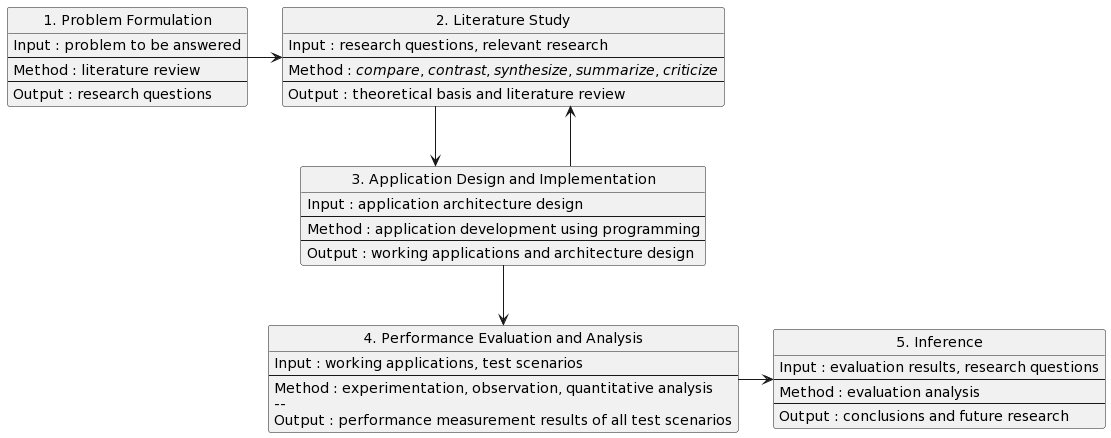
\includegraphics[width=1\textwidth]{assets/diagrams/research-stages.png}
	\caption{Research stages.}
	\label{fig:research-stages}
\end{figure}

In the first stage, problem formulation, existing problems are used with the help of literature review to produce research questions that are answered in the conclusion of this study. In the second stage, literature study, relevant research is used to define/create the basis of this research. The methods used in the literature study stage are the following: compare, contrast, synthesize, summarize, and criticize which helps to get the theoretical foundation and literature review of this research.

In the third stage, application design and implementation, the web application architecture is designed and implemented to be used as a common variable for testing to be done. The configuration of geo-distributed Kubernetes clusters and Istio service mesh is also done in this stage. In the fourth and penultimate stage, testing is done, and each testing scenario is evaluated to answer research questions and acquire a conclusion for this study, which is done in the final stage.

% \section{Application Infrastucture Design}
% \label{sec:applicationInfrastructureDesign}
% Two areas that need to be configured in the complete web application are the application server itself and the geo-distributed Kubernetes clusters. The application is a two-tiered application consisting of a server and database tier. The client tier is omitted from the application itself but instead is represented by the Vegeta load testing tool. The server is a REST API that communicates with a database and simply returns the cluster name of where the responding server is located. The server is then containerized using Docker and uploaded to Docker Hub to be used by Kubernetes. This separation of concern between application development and infrastructure development allows for concurrent progress to be made between the two different areas and is a big reason why Docker and Kubernetes are widely adopted.

% The next step after application configuration is the geo-distributed clusters configuration. The two different configurations are MCS with MCI and Istio / ASM. For the MCS with MCI configuration, the server service is deployed as a MultiClusterService custom resource and is routed by the MultiClusterIngress custom resource which allows cross-cluster communication. A virtual IP address is then created which uses a Google Cloud Load Balancer that routes traffic to the nearest cluster. The infrastructure for the MCS with MCI geo-distributed Kubernetes clusters can be seen in \autoref{fig:infra-mcs-mci}.

% \begin{figure}
% 	\centering
% 	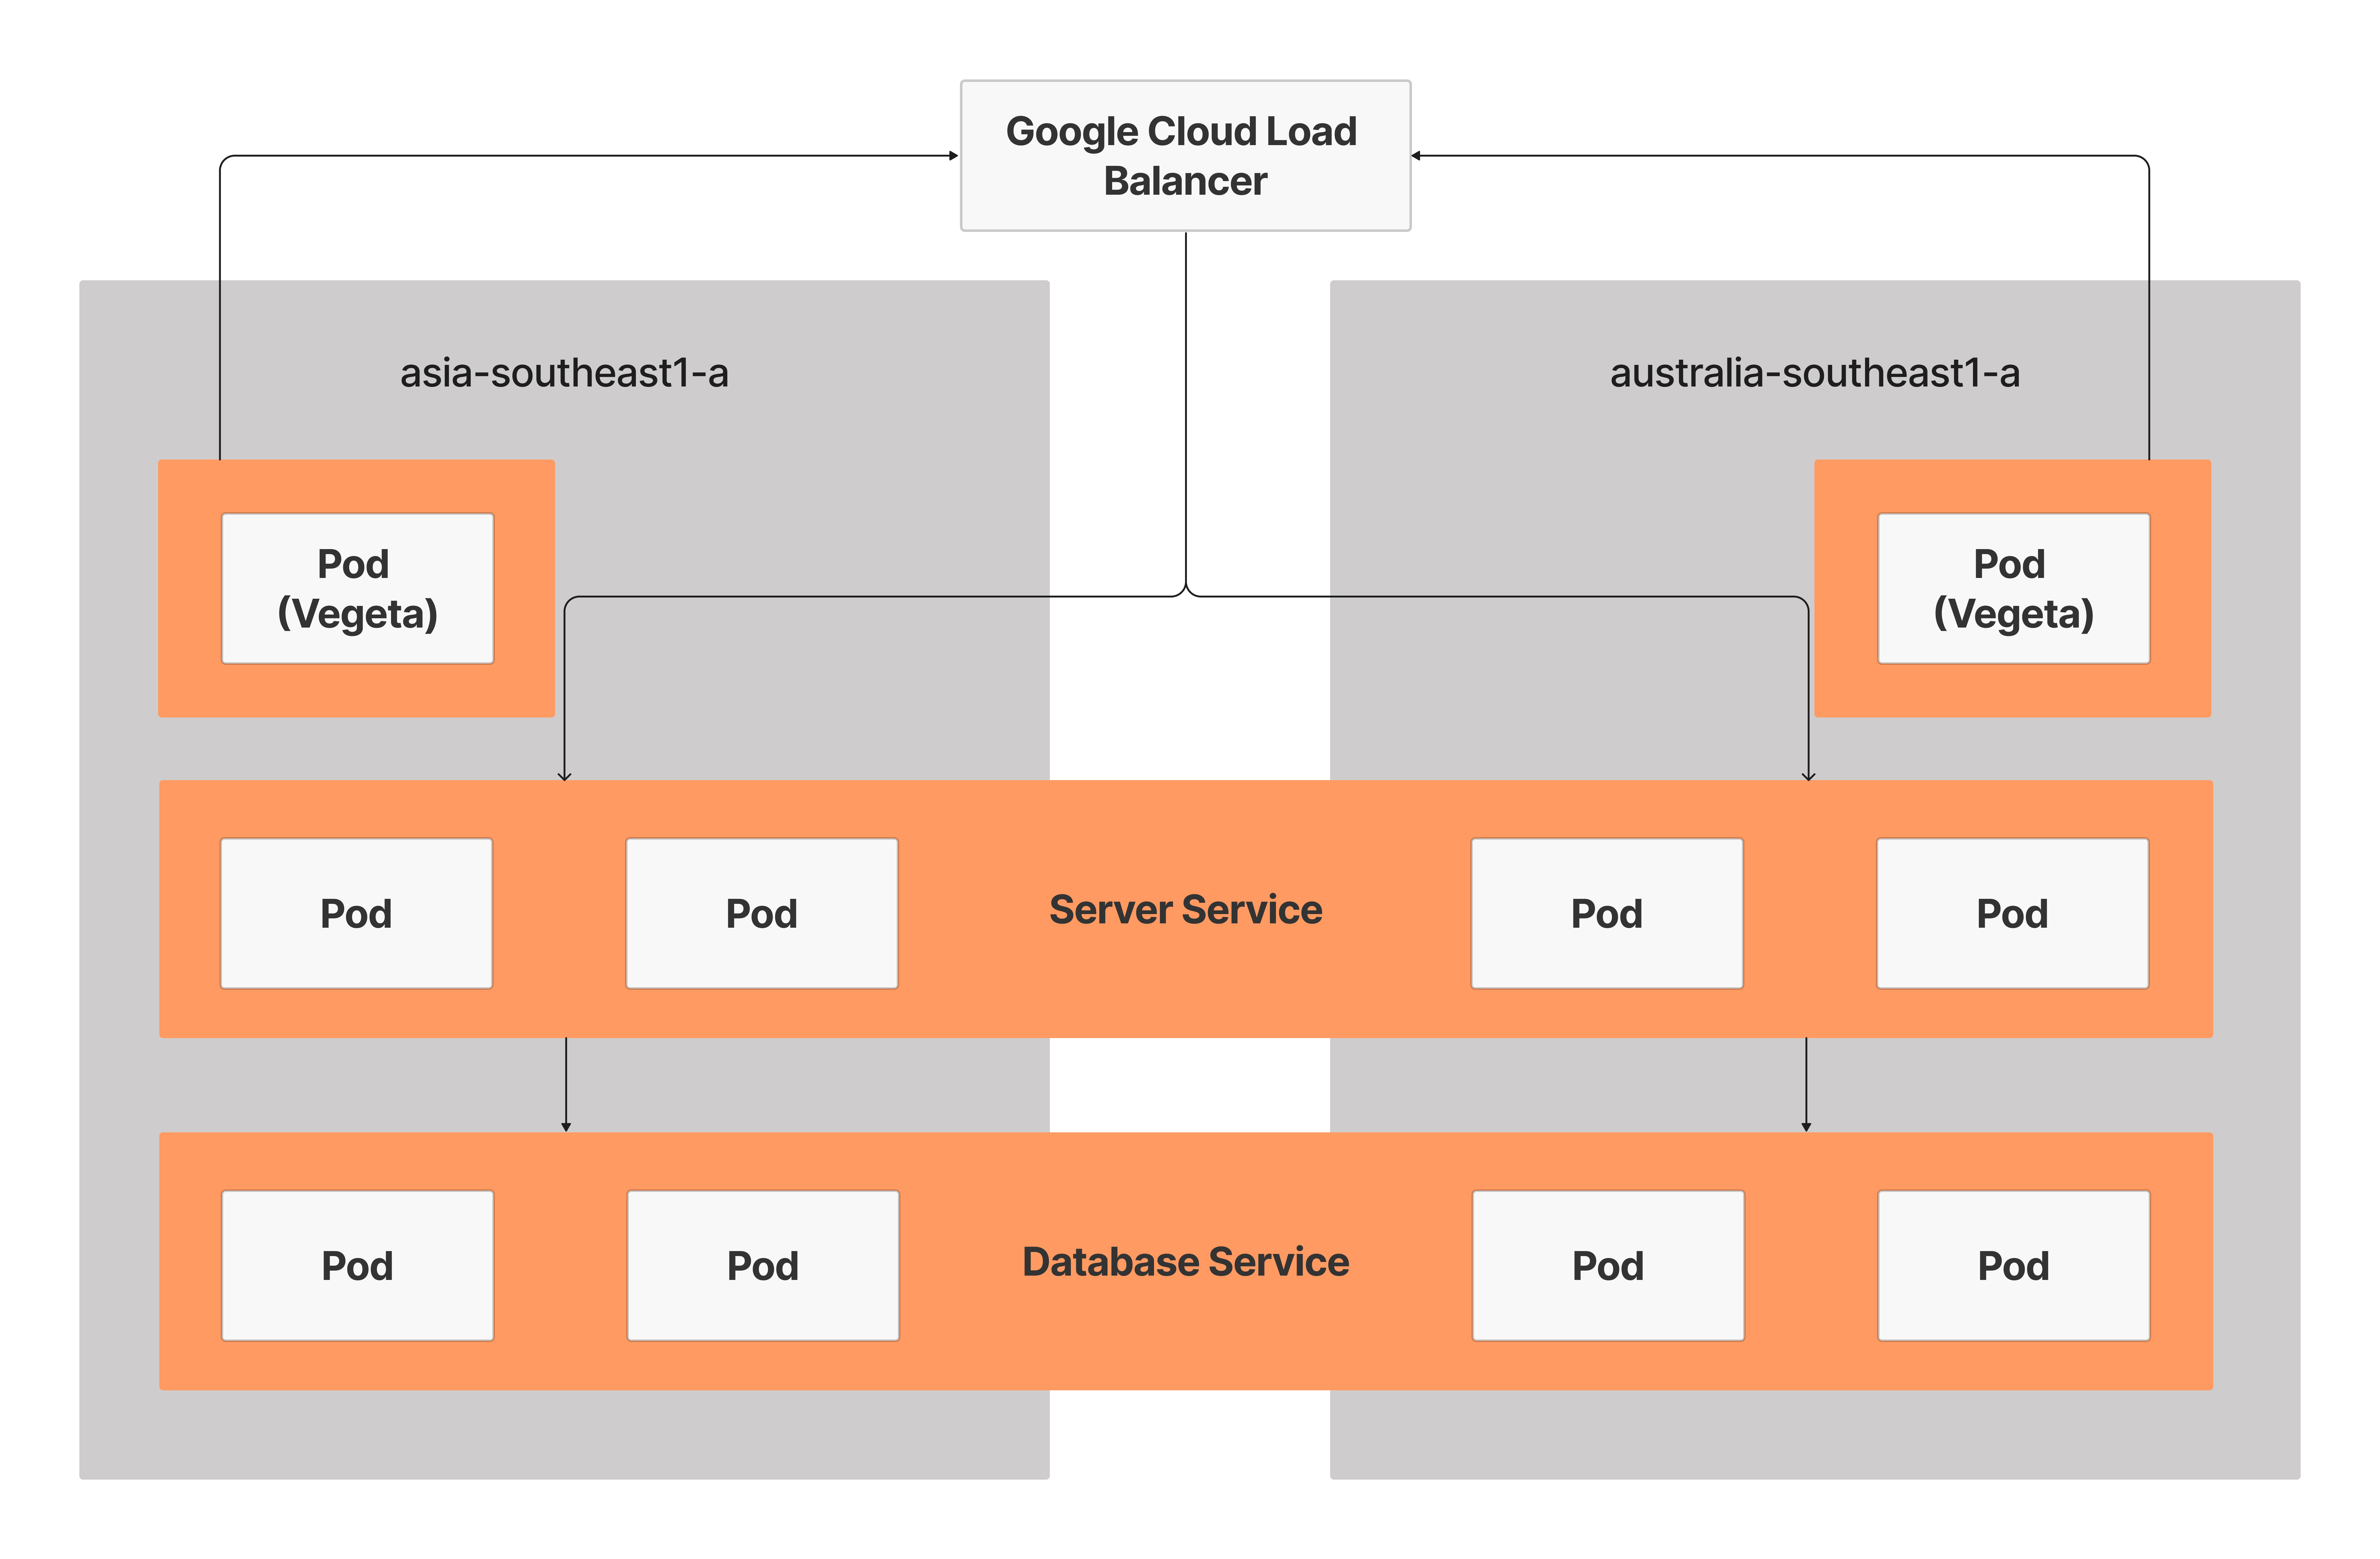
\includegraphics[width=1\textwidth]{assets/diagrams/infra-mcs-mci.png}
% 	\caption{Geo-distributed Kubernetes clusters infrastructure on the MCS with MCI configuration.}
% 	\label{fig:infra-mcs-mci}
% \end{figure}

% For the Istio / ASM configuration, each cluster is installed with Istio control and data plane which enables automatic envoy proxy injection to each pod. A DestinationRule resource is then deployed to configure locality load balancing which routes traffic to the nearest cluster. The Vegeta load testing pod is deployed in every region to simulate a request call from each region. The database layer can't be load balanced directly, as a database instance is needed on the server runtime. An approach to counter this is to have a dedicated data layer which is a server for each database instance. The infrastructure for the Istio / ASM geo-distributed Kubernetes clusters can be seen in \autoref{fig:infra-istio}.

% \begin{figure}
% 	\centering
% 	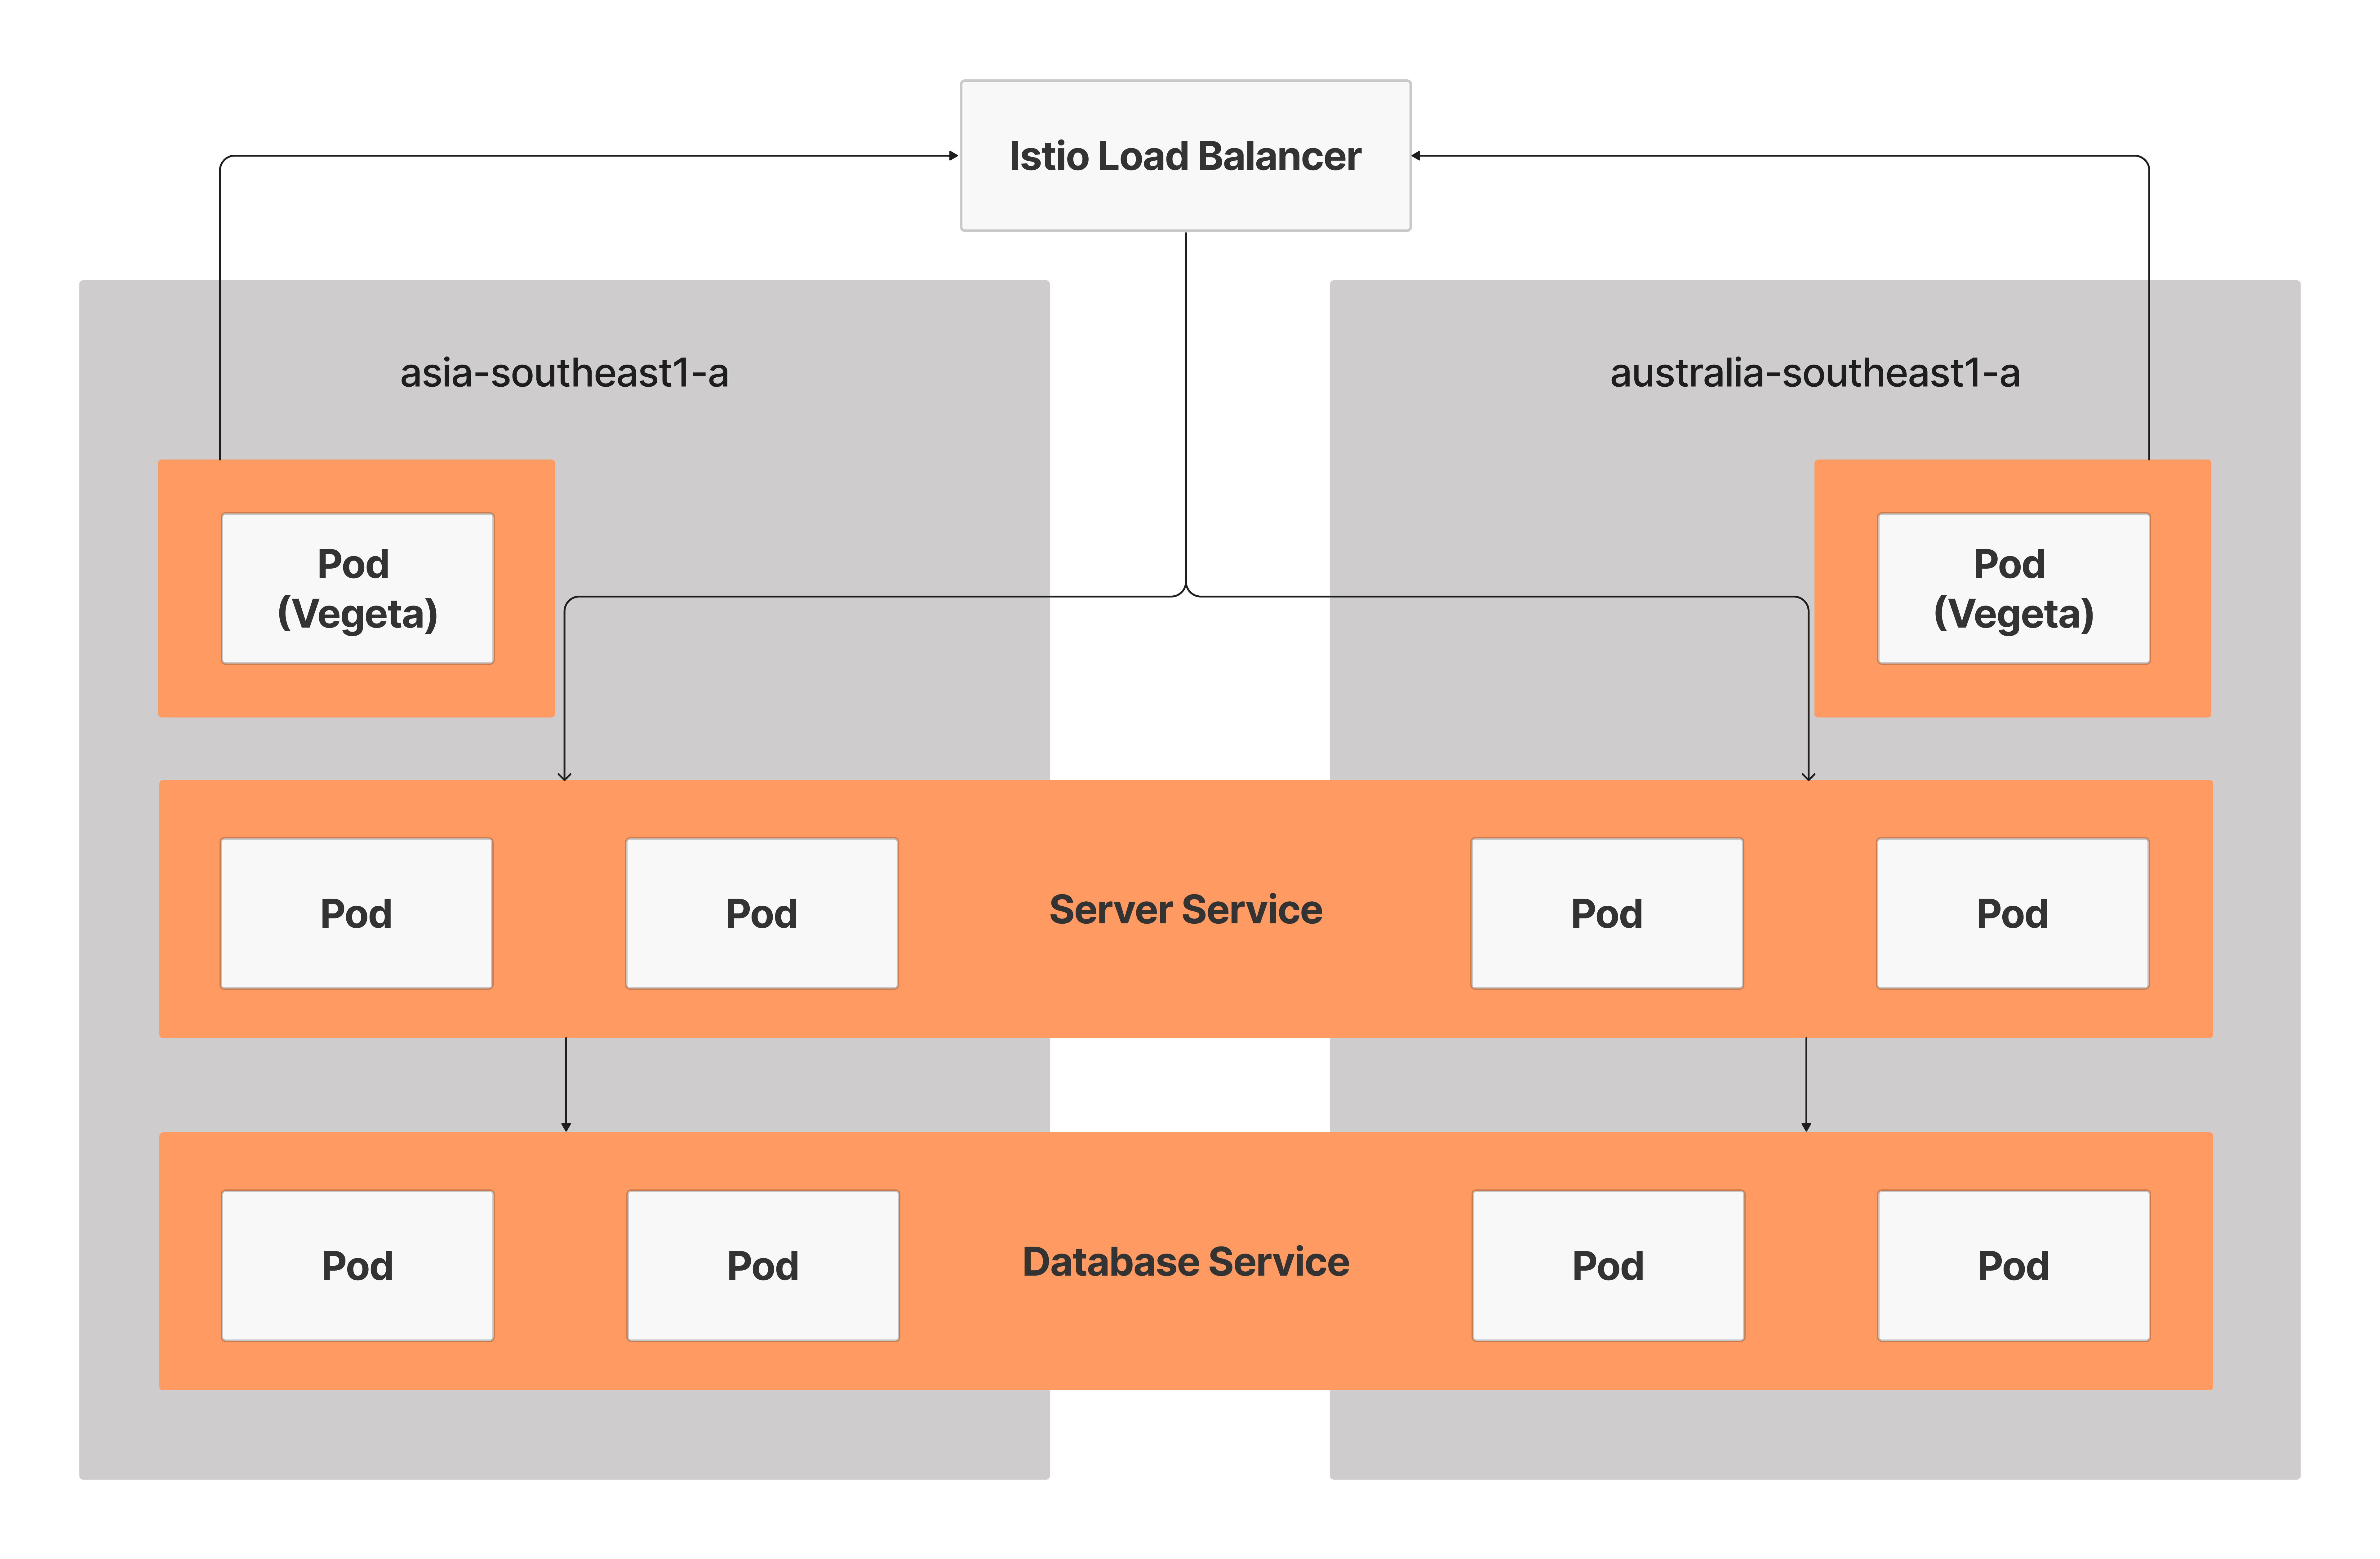
\includegraphics[width=1\textwidth]{assets/diagrams/infra-istio.png}
% 	\caption{Geo-distributed Kubernetes cluster infrastructure on Istio / ASM configuration.}
% 	\label{fig:infra-istio}
% \end{figure}

\section{Testing Scenarios}
\label{sec:testingScenarios}
In the testing scenario, load testing and stress testing are done to evaluate the performance of each geo-distributed cluster configuration. Being a quantitative research and quantitative experimentation, there are variables that need to be established. The independent variables are the different geo-distributed Kubernetes cluster configurations, load balancer algorithm, and the different requests per second configured during performance testing. For each geo-distributed cluster configuration, testing is done by increasing the RPS after each test case. Each test case occurs for 5 seconds to simulate a short period where a server experiences high traffic, for example during a flash sale. The RPS used in the testing configuration are 10, 50, and 100 where 100 is the upper limit chosen from the number of errors that occurred during preliminary tests. The independent variables are shown in \autoref{table:combined-config}.

% \begin{table}
% \centering
% \begin{tabular}{|c|c|}
% \hline
% Geo-Distributed Cluster Configuration                      & Load Balancer \\ \hline
% MCS with MCI                    & Geo-Aware                    \\ \hline
% Istio / ASM                 & Round Robin                              \\ \hline
% Istio / ASM                  & Geo-Aware                   \\ \hline
% \end{tabular}
% \caption{Configuration of geo-distributed clusters}
% \label{table:geo-distributed-cluster-test-config}
% \end{table}

% \begin{table}
% \centering
% \begin{tabular}{|c|}
% \hline
% Region Request Origin Configuration                      \\ \hline
% asia-southeast1-a \\ \hline
% australia-southeast1-a \\ \hline
% \end{tabular}
% \caption{Configuration of region request origin}
% \label{table:region-origin-test-config}
% \end{table}

% \begin{table}
% \centering
% \begin{tabular}{|c|}
% \hline
% Requests Per Second (RPS) Configuration                       \\ \hline
% 10                                        \\ \hline
% 50                                               \\ \hline
% 100                                    \\ \hline
% \end{tabular}
% \caption{Configuration of requests per second (RPS)}
% \label{table:rps-test-config}
% \end{table}

% \begin{table}[htbp]
\begin{table}
\centering
\caption{Configuration of geo-distributed cluster method, load balancer, and requests per second}
\begin{tabular}{|c|c|c|}
\hline
Geo-Distributed Cluster Method & Load Balancer & Requests Per Second (RPS) \\ \hline
& Multi-Cluster Geo-Aware & 10 \\ \cline{3-3}
MCS with MCI & & 50 \\ \cline{3-3}
& Single Cluster & 100 \\ \hline
& Multi Cluster Geo-Aware & 10 \\ \cline{3-3}
Istio / ASM & & 50 \\ \cline{3-3}
& Single Cluster & 100 \\ \hline
\end{tabular}
\label{table:combined-config}
\end{table}

The product of all of the different variables results in 12 different testing scenarios, which are repeated three times for each scenario to reduce variability. The dependent variables are evaluation metrics which include the number of requests, latency, and success ratio. In addition, each test scenario is executed independently from one another to avoid the effects of external variables. The test implementation details can be seen in \autoref{sec:load-testing-implementation}.

\section{Evaluation Metrics}
\label{sec:evaluationMetrics}
% Performance is the main metric to be evaluated and can be defined in several ways. In every test scenario, the following metrics are gathered to analyze web performance:
% \begin{itemize}
%     \item Requests      [total, rate, throughput]
%     \item Duration      [total, attack, wait]
%     \item Latencies     [min, mean, 50, 90, 95, 99, max]
%     \item Success       [ratio]
%     \item Status Codes  [code:count]
% \end{itemize}

When analyzing web performance, several metrics can define an application's performance. These metrics include the number of requests made which is evaluated in terms of total requests, request rate, and throughput. Additionally, latency is another metric that tells us the amount of time taken from sending a request until the first byte of the response is received and is tracked in the form of the minimum latency, the maximum latency, the mean latency as well as 50th, 90th, 95th and 99th percentile. 

Aside from performance, the purpose of having a high number of requests per second in the test scenario is to evaluate the server's capability to return to a healthy state after experiencing a server failure. The success ratio provides insight into the number of successful responses, defined by having a response code between 200 and 400 (non-inclusive), and is used to determine a configuration's resiliency.

